\section{Methodology}

The intention of this work is to propose a system for a mobile robot in order to plan its movements without any map knowledge on the environment. Its translation function is defined as:
\begin{equation}
v_t = f(x_t, p_t, v_{t-1})
\end{equation}
where $x_t$ is the observation from the raw sensor information, $p_t$ is the relative position of the target, and $v_{t-1}$ is the velocity of the mobile robot in the last time step.
All variables specified, previously, can be defined as the current state $s_t$ of the mobile robot.
With this model it is possible to get the actions that the robot will make, given its current state.
However, it is needed to ensure a minimum reading frequency of the input data to control the movement of the robot because if the robot get a slow read frequency of the inputs it cannot react to an obstacle in the trajectory to a target. In this way, the robot can react to new states quickly.
This method was first explored by Tai et al. \cite{tai2017virtual}.

\subsection{Network Structure}

Once the system of state and actions has been defined, it is possible to create a SAC network capable of resolving the problem.
The SAC network has 14 inputs as presented in Fig. \ref{fig:entradaESaida}, in which 10 corresponds to the laser range findings, 2 corresponds to the previous linear and angular velocity, and the other 2 corresponds to the relative position and angle of the mobile robot to the target.
The sample of the laser range findings are between $-90$ and $90$ degrees in relation to the robot. The output of the network is the action of linear and angular velocity that will be applied on the mobile robot.

\begin{figure}[htbp]
\centerline{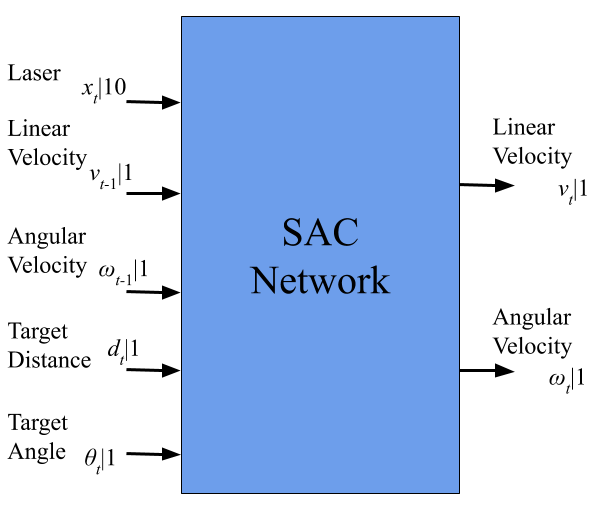
\includegraphics[width=\columnwidth]{images/output_and_input.png}}
\caption{SAC network inputs and outputs.}
\label{fig:entradaESaida}
\end{figure}

The network structure of the SAC is shown in Fig \ref{fig:projetointegrador}. 
The actor-network has as input the current state of the mobile robot followed by 4 fully-connected neural networks layers with 512 nodes.
This input of the networks is transformed on the linear and angular velocity that will be the commands sent to the motor of the mobile robot. 
The action range is constrained between $(-1,1)$ and the hyperbolic tangent function $(tanh)$ is used as activation function.
The outputs of the action are then changed for the linear velocity that varies between $0$ to $0.22$ $m/s$ and the angular velocity be between $-2$ to $2$ $rad/s$ on the TurtleBot3 robot version Burger.


\begin{figure}[htbp]
\centerline{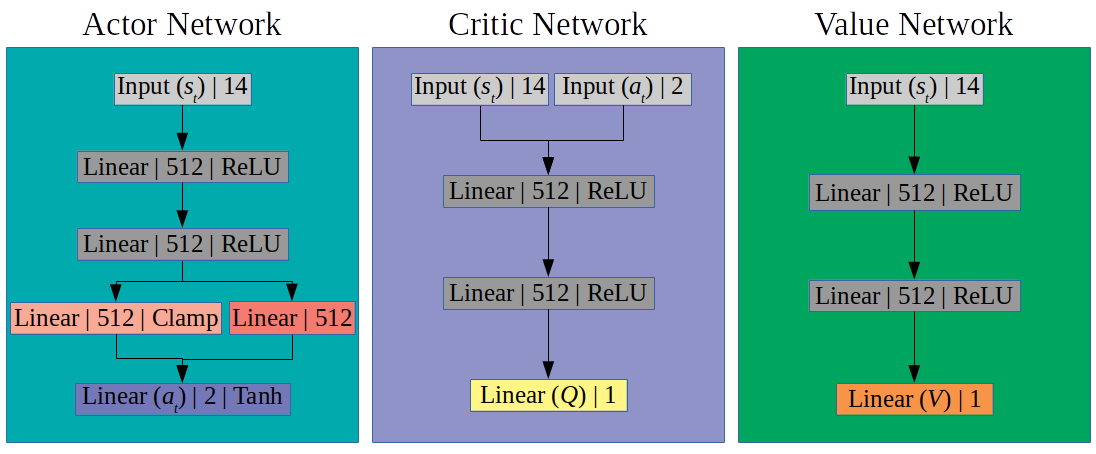
\includegraphics[width=\columnwidth]{images/structure_sac.png}}
\caption{SAC network structure model.}
\label{fig:projetointegrador}
\end{figure}

In the critic-network, the Q-value of the current state and action are predicted.
And in the value-network, the value of the current state is predicted.
The two networks use only 2 fully-connected neural networks layers to process the input state.
The Q-value and the value of the current state is activated through a linear activation function:
\begin{equation}
y = kx +b
\end{equation}
where $x$ is the input of the last layer, $y$ is the predicted Q-value or the predicted value of the current state, and $k$ and $b$ are the trained weights and bias of this layer, respectively.

\subsection{Reward Function}

Once the environment has been defined it is possible to simulate a controlled mobile robot for a navigation task.
It is necessary to define the reward and penalty system to the Deep-RL network.
Remembering that the rewards and penalties are attributed numbers passed to the intelligent agent.
So, the network will make a feedforward and backpropagation step in order to learn the hyperparameters.

There are four different conditions for the reward system that presented better results for the resolution of the problem and are the following:
\begin{equation}
r (s_t, a_t) = 
\begin{cases}
r_{arrive} \ \textrm{if} \ d_t < c_d
\\
r_{collide} \ \textrm{if}\ min_x < c_o
\\
c_{r1}(d_{t-1} - d_t) \ \textrm{if} \ (d_{t-1} - d_t) > 0
\\
c_{r2} \ \textrm{if} \ (d_{t-1} - d_t) \leq 0
\end{cases}
\end{equation}

If the robot gets to the target through threshold checking $c_d$, a positive reward $(r_{arrive})$ is given, but if the robot collides with an obstacle through a minimum range readings checking, a negative reward $(r_{collide})$ is given.
Both conditions are sufficient to end the training episode.
Otherwise, the reward is based on the distance difference from the target compared to the last time step $(d_{t-1} - d_t)$. 
If this difference is positive the reward given is the distance traveled multiplied by the hyperparameter $(c_{r1})$, and if the distance is negative is used the hyperparameter $(c_{r2})$.
This motivates the mobile robot to get closer to the target position and encourages it to avoid the obstacles in the environment.

% \subsection{Positioning capture in real environments}

% After training the SAC network through simulation, it will be tested in a real scenario.
% The Turtlebot3, version Burger, will be used to perform this test.
% It will be necessary to obtain the angle and distance of a target for the network to complete its goal.
% So it was setup a camera in the ceiling to extract this information.

% Firstly, the essential points positions to extract the angle and distance are taken from the image.
% These positions include the target, left and right side of the robot, and three points to be a distance reference parameter.
% Fig. \ref{fig:pixel_to_meter} shows a frame of the scenario in which there were used different colored circles to identify the relevant points.
% The yellow circle was attached as the target, the blue to the left side of the robot, the red to the right side and the three green circles were used as reference parameter to calculate the distance.

% \begin{figure}[htbp]
% \centerline{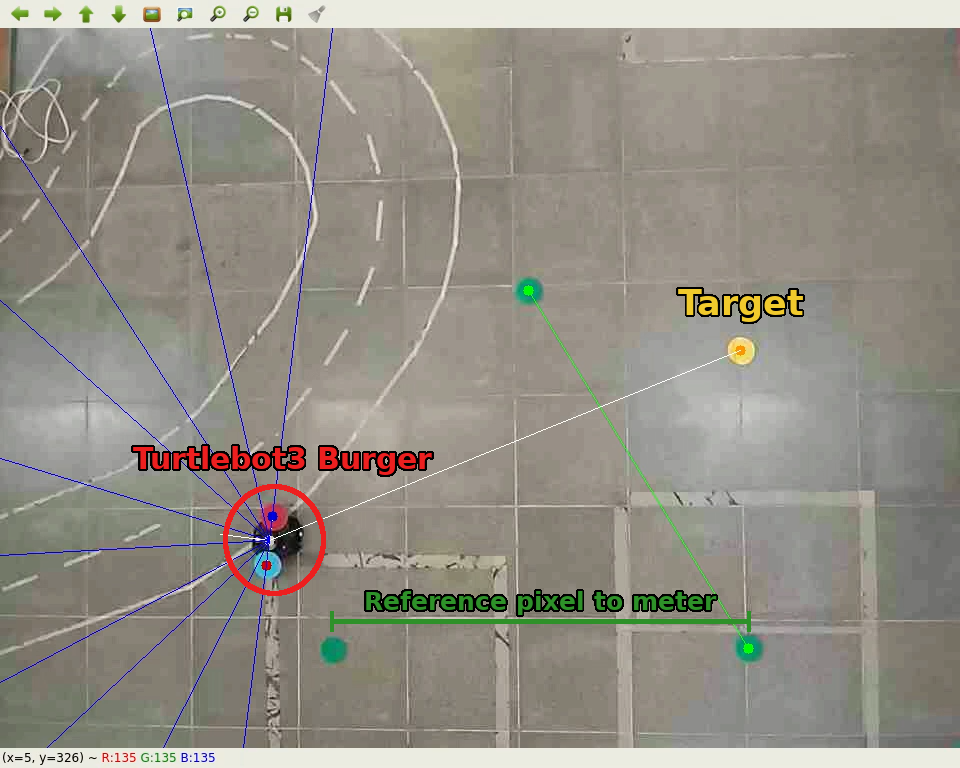
\includegraphics[width=6cm]{images/pixel_to_meter.png}}
% \caption{Real environment relevant points}
% \label{fig:pixel_to_meter}
% \end{figure}


% After the points were extracted from the center of the circles, it is possible to calculate the two necessary SAC network inputs.
% So, it is necessary to figure out the vector distance that connects the center of the Turtlebot3 to the target point, and the vector direction which represents the direction of the robot.
% The distance and angle between the mobile robot and the target are calculated frame by frame, and it is used as the necessary inputs of the SAC network simultaneously.



%aqui vou escrever mais 
%The center of green circles have a predefined distance from each other, what permits the calculation of robot and target distance by converting the pixel distance of the image to the distance in meters.
%aqui tbm





%After the points were extracted from the center of the circles, it is possible to calculate the two necessary SAC network inputs.
%So, it is necessary to figure out the vector $distance$ that connects the center of Turtlebot3 to the target point, and the vector $direction$ which represents the direction of robot.
%The vector $direction$ starts from the center of Turtlebot3, which is equal to the midpoint of the blue and red points.
%The blue and red circles are on left and right sides of the mobile robot, respectively.
%With this it is possible to determine the front of the robot.

%aqui vou escrever mais 
%The center of green circles have a predefined distance from each other, what permits the calculation of robot and target distance by converting the pixel distance of the image to the distance in meters.
%aqui tbm



% e aeee
%acabei de perder meia hora no face AAAAAAA
% cara, na escrita n me dou mt bem, mas vou escrevendo o q vem na cabeça e após a gente estrutura melhor
% faz isso mesmo meu KKKK eu sou meio travado na vdd mas to tentando (bem travado)
% a ideia é meter o louco e escrever tudo que vem na mente
% isso vem com a pratica SAUHSUAS, 
% pode se sentir a vontade pra mudar as coisas.
% só modifiquei pq achei melhor - ficou melhor assim msm ;)
% o que tu conseguir escrever eu e o professor gamarra corrigimos depois


%qual tu pensa a imagem pra colocar nessa subsection ae
%um frame com o alvo indicado, pixel meter parameter tb, e o robo? q nem o video do face? ---> meu acho que pode ser só uma imagem que contenha o robo, a referencia e tals (pode ser do primeiro ambiente que a gente tinha feito) ai tu explica através dela - OK

%coloquei a imagem do grafico com os obstáculos no drive, acho q ficou ok ---> eu vi, tá top na real - :D
% amanhã vou pegar pra escrever nos resultados, tava editando o modelo mais hj - azulzinho topi --> e as imagens pra ficarem melhor tbm
% vou pegar pra dormir aqui na real, flws o/// falooooow veéeei até amanhã
